%%
%% $Id$
%%
%% Copyright (c) 2007-2008 Christian Fehler
%% Copyright (c) 2007-2008 Benjamin Mies
%%


%### removes texlipse warnings


\myslide{Automaten}
{
    \begin{itemgroup}{}
	\item Graphenansicht
	\item Übergangs-Tabelle
	\item Wort-Navigation
	\item Erreichbare Zustände
	\item Konvertierung
	\item Minimierung
	\end{itemgroup}

	\vfill{}
}


\myslide{Automaten - Graphenansicht}
{
    \begin{itemgroup}{}
	\item Orientierung an der Vorlesung
	\item Normale Zustände werden durch Kreis mit Namen in der Mitte dargestellt
	\begin{itemgroup}{}
		\item Startzustände haben zusätzlich einen mit Start beschrifteten Pfeil
		\item Akzeptierende Zustände haben zusätzlich einen doppelten Rahmen
	\end{itemgroup}
	\item Übergänge werden als Pfeil mit Übergangsmenge dargestellt
	\end{itemgroup}

	\vfill{}
}


\myslide{Automaten - Graphenansicht}
{
  \begin{center}
    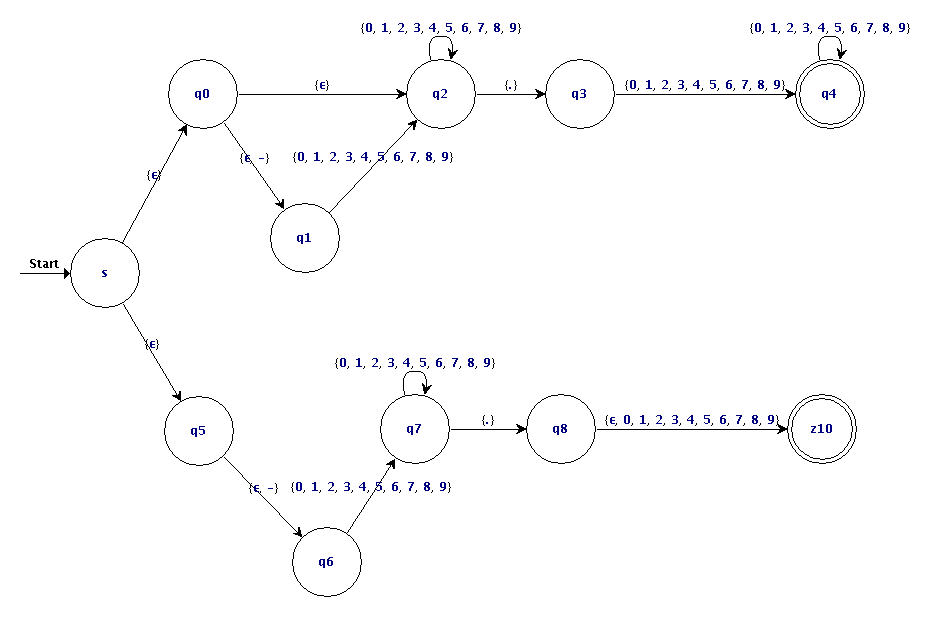
\includegraphics[height=14cm]{../images/enfa_example.png}
  \end{center}
}


\myslide{Automaten - Übergangs-Tabelle}
{
    \begin{itemgroup}{}
	\item Nicht nur graphische Bearbeitung eines Automaten
	\item Schnellere Änderungen an einem Automaten
    \end{itemgroup}

    \begin{itemgroup}{Lösung}
	\item Editierbare Tabelle
	\item Übergänge werden angelegt, gelöscht oder modifiziert
	\end{itemgroup}
    
    \vfill{}
}


\myslide{Automaten - Übergangs-Tabelle}
{
  \begin{center}
    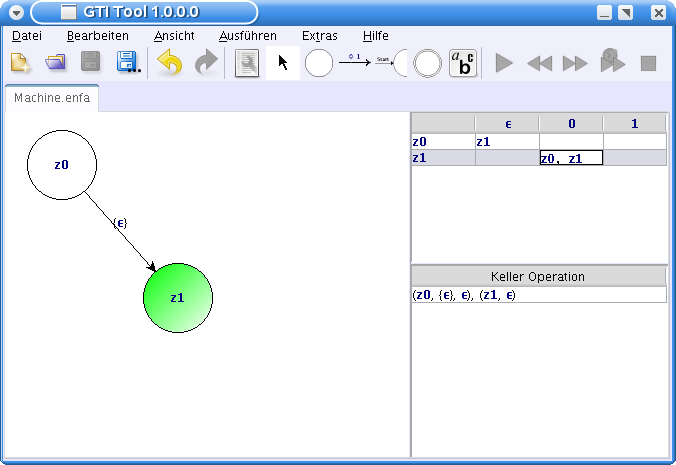
\includegraphics[height=14cm]{../images/machine_table.png}
  \end{center}
}


\myslide{Automaten - Wort-Navigation}
{
    \begin{itemgroup}{}
	\item Eingabe eines Wortes
	\item Zeichenweise Navigation durch das Wort
	\item Aktive Zustände und Übergänge werden hervorgehoben
	\item Es wird angezeigt wie weit das Wort bereits gelesen wurde
	\end{itemgroup}

	\vfill{}
}


\myslide{Automaten - Wort-Navigation}
{
  \begin{center}
    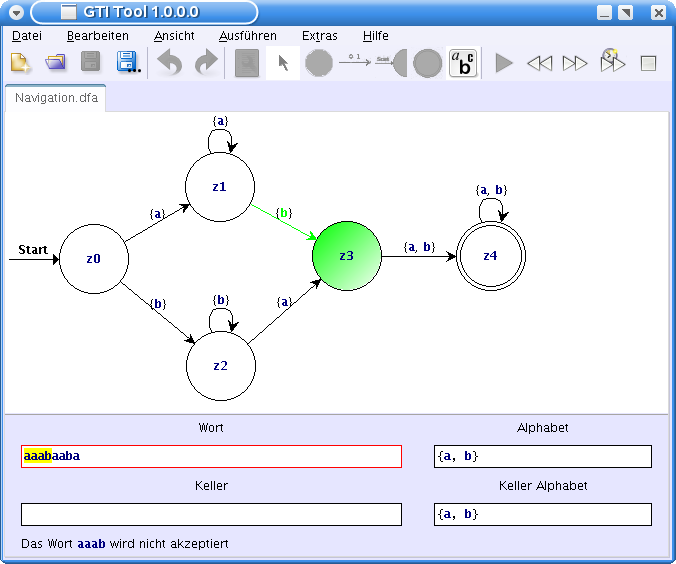
\includegraphics[height=14cm]{../images/dfa_navigation.png}
  \end{center}
}


\myslide{Automaten - Wort-Navigation}
{
    \begin{itemgroup}{}
	\item Nicht deterministischer Kellerautomat
	\item Auswahl des nächsten Übergangs nicht eindeutig
    \end{itemgroup}

    \begin{itemgroup}{Lösung}
	\item Falls deterministisch Übergang verwenden
	\item Sonst Benutzer auswählen lassen
	\end{itemgroup}
    
    \vfill{}
}


\myslide{Automaten - Wort-Navigation}
{
  \begin{center}
    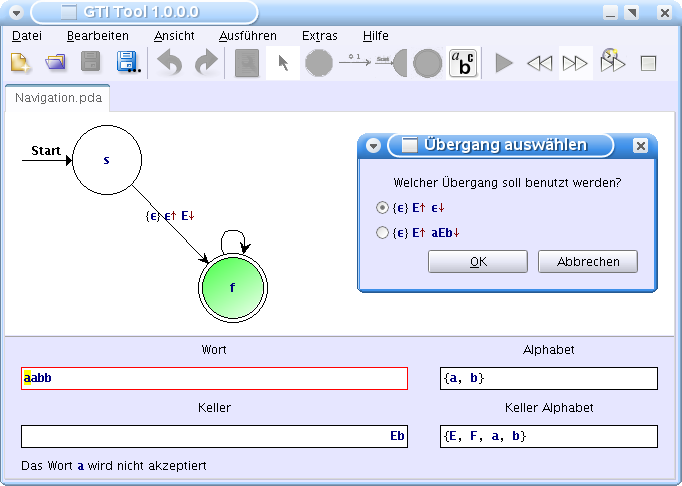
\includegraphics[height=14cm]{../images/grammar_pda.png}
  \end{center}
}


\myslide{Automaten - Erreichbare Zustände}
{
    \begin{itemgroup}{}
	\item Erreichbare Zustände erkennen
	\item Unerreichbare Zustände entfernen
	\item Wird bei der Minimierung verwendet
    \end{itemgroup}

    \begin{itemgroup}{Lösung}
	\item Verwendung der Breitensuche
	\item Nicht erreichbare Zustände werden nicht markiert
	\item Ergebnis: Automat mit nur erreichbaren Zuständen
	\end{itemgroup}
    
    \vfill{}
}


\myslide{Automaten - Erreichbare Zustände}
{
  \begin{center}
    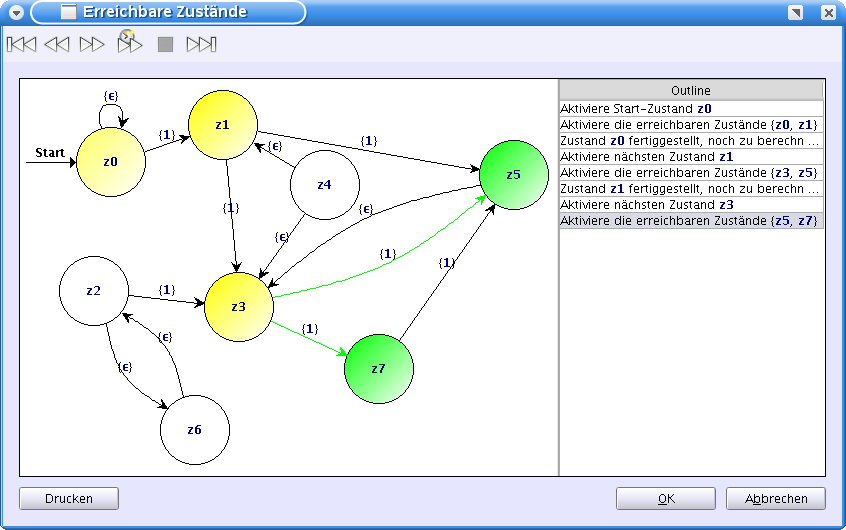
\includegraphics[height=14cm]{../images/reachable_states.png}
  \end{center}
}


\myslide{Automaten - Konvertierung}
{
    \begin{itemgroup}{}
	\item Konvertierung NDEA $\to$ DEA
    \item Konvertierung $\epsilon$-NDEA $\to$ DEA
    \item Konvertierung $\epsilon$-NDEA $\to$ NDEA
    \end{itemgroup}

    \begin{itemgroup}{Lösung}
	\item Für jeden Zustand und jedes Symbol überprüfen
	\begin{itemgroup}{}
	  \item Welche Zustände sind von dem Zustand mit dem Symbol erreichbar
	  \item Übergang mit dem Symbol zu dem neuen Zustand anlegen
	  \item Gegebenenfalls den neuen Zustand anlegen
	\end{itemgroup}
	\item Potenzmengen Konstruktion: Alle Zustände direkt anlegen
	\end{itemgroup}
    
    \vfill{}
}


\myslide{Automaten - Konvertierung}
{
  \begin{center}
    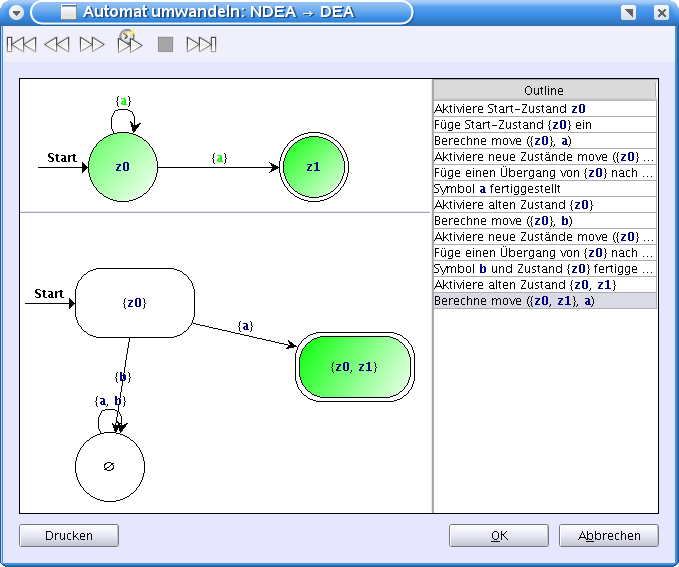
\includegraphics[height=14cm]{../images/convert_to.png}
  \end{center}
}


\myslide{Automaten - Minimierung}
{
    \begin{itemgroup}{}
	\item Nicht erreichbare Zustände entfernen
	\item Einteilung in zwei Äquivalenzklassen
		\begin{itemgroup}{}
		\item Akzeptierende Zustände
		\item Nicht akzeptierende Zustände
		\end{itemgroup}
	\item Verfeinern der Äquivalenzklassen
	\item Jede Äquivalenzklasse repräsentiert einen Zustand in dem minimalen
	Automat
	\end{itemgroup}
	
	\vfill{}    
}


\myslide{Automaten - Minimierung}
{
  \begin{center}
    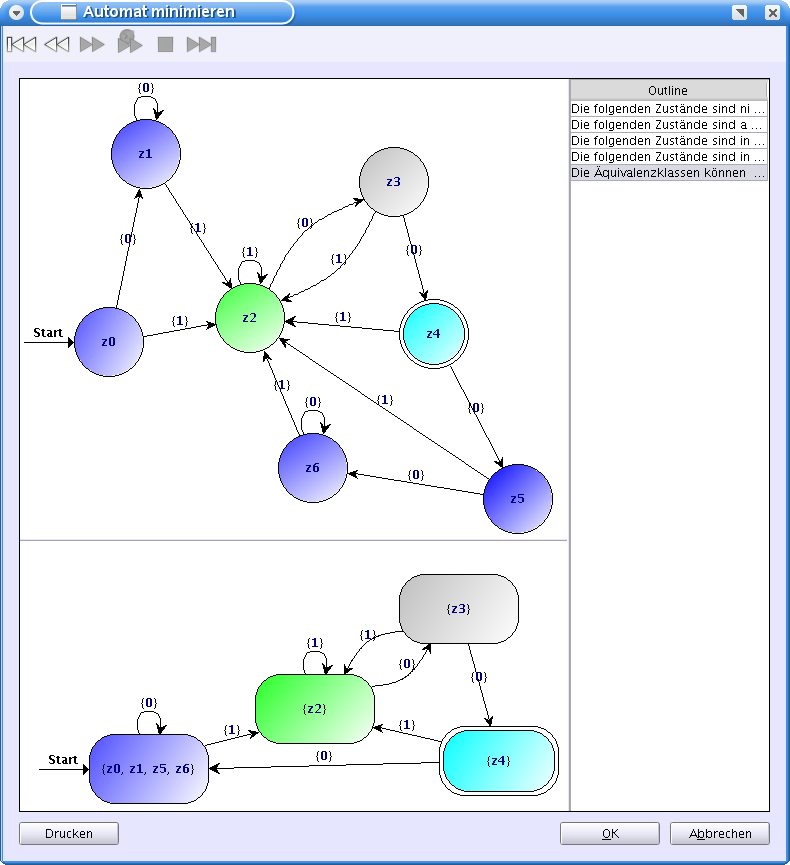
\includegraphics[height=14cm]{../images/minimize.png}
  \end{center}   
}


%### removes texlipse warnings
